Dense convolutional neural networks address a problem of deep \ac{CNN}s. \autocite{Huang.2017}
\blockquote[\cite{Huang.2017}]{As information about the input or gradient passes through many layers, it can vanish and \enquote{washout} by the time it reaches the end (or beginning) of the network.
}
Dense convolutional neural networks address this problem by connecting all layers with each other, see Figure \ref{fig:denseconv}. The input of a layer is the concatenation of the original input and all outputs of previous layers. This way, information flow between layers in the network is encouraged. \autocite{Huang.2017}
\begin{figure}[H]
	\centering
	
%\cube{x offset}{y offset}{width}{height}{depth}{color}{fillcolor}
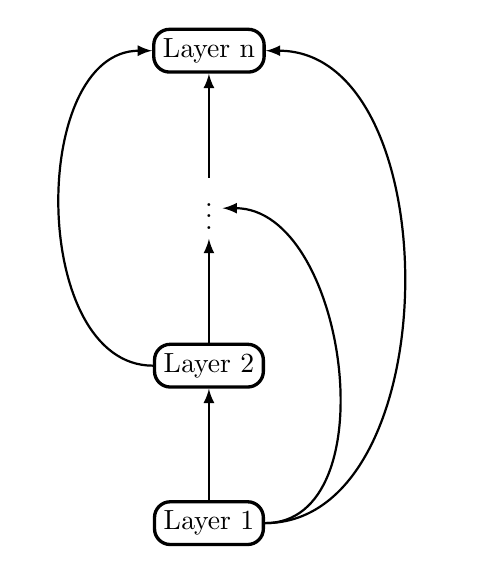
\begin{tikzpicture}[
	cell/.style={
		rectangle, 
		rounded corners=2mm, 
		draw,
		very thick,
		align=center,
	},
	ArrowC1/.style={% Arrows with rounded corners
		rounded corners=.25cm,
		thick,
	},
]

\node[cell] (l1) at (0,0) {Layer 1};
\node[cell] (l2) at (0,2) {Layer 2};
\node (dots) at (0,4) {$\vdots$};
\node[cell] (ln) at (0,6) {Layer n};

\draw[-latex, ArrowC1] (l1) -- (l2);
\draw[-latex, ArrowC1] (l2) -- (dots);
\draw[-latex, ArrowC1] (dots) -- (ln);

\draw[-latex, ArrowC1] (l1) to[out=0, in=0] (ln);
\draw[-latex, ArrowC1] (l1) to[out=0, in=0] (dots);

\draw[-latex, ArrowC1] (l2) to[out=-180, in=180] (ln);

	
\end{tikzpicture}
	\caption{Dense Convolutional Neural Network (own figure)}
	\label{fig:denseconv}
\end{figure}
\par
An additional, counter-intuitive effect of dense convolutional neural networks is that they require fewer parameters. 
Traditional neural networks pass information from layer to layer. Consequently, layers need to learn what information needs to be added and preserved. Dense convolutional neural networks explicitly distinguish between added and preserved information. Features are reused. Thus, they do not need to learn which information to preserve. Therefore, they need fewer parameters. \autocite{Huang.2017}
\par
The best-performing dense convolutional neural network found in the course of the literature review is the $264$ layer version of \cite{Huang.2017}'s DenseNet, called DenseNet-264.
The input of DenseNet-264 is a $224$-by-$224$-pixel, \ac{RGB} image. The output of DenseNet-264 comprises the probabilities of the $c$ target classes. 
DenseNet-264 is comprised of convolutional layers followed by $1$ dense layer. \autocite{Huang.2017}
\par
The convolutional layers have a stride of $1$ and a padding preserving spatial dimensions.
The first convolutional layer has $64$ kernels of size $7$ and a stride of $2$. It is followed by batch normalization, \ac{ReLU} activation function, and max pooling. Max pooling is applied with a pooling size of $3$, a pooling stride of $2$, and a padding preserving spatial dimensions. \autocite{Xie.2017}
The remaining convolutional layers are arranged in $4$ dense blocks and $3$ transition layers. A transition layer is applied between each dense block.
After the last dense block batch normalization, \ac{ReLU} activation function, global average pooling, and a dense layer are applied.
The dense layer has $c$ neurons and uses the softmax activation function. \autocite{Huang.2017}
\par
A dense block consists of $L$ convolutional blocks. All convolutional blocks are connected with each other. In consequence, the input of the $l$th convolutional block is the concatenation of the input of the dense block and the outputs of all previous layers. The output of the dense block is the concatenation of the input of the dense block and the outputs of all convolutional blocks of the dense block. Therefore, inside the dense block, the spatial dimensions of all feature maps are the same. A convolutional block consists of $2$~convolutional layers. The first layer has $128$~kernels of size~$1$. The second layer has $32$~kernels of size~$3$. Batch normalization and \ac{ReLU} activation function are applied before each convolution. The configurations of each dense block are outlined in Table \ref{tab:densenet}. \autocite{Huang.2017}
\par
A transition layer reduces the number and spatial dimensions of the feature maps.
A transition layer consists of the sequence batch normalization, \ac{ReLU} activation function, convolution, and average pooling. The convolution is used to reduce the number of feature maps by factor $0.5$. Hence, the convolution has $0.5 \cdot d$ kernels of size~$1$ with $d$ being the initial number of feature maps. The average pooling is used to reduce the spatial dimensions of the feature maps. The pooling is of size $2$ and has a stride~of~$2$. \autocite{Huang.2017}
\par
The whole configuration of DenseNet-264 is outlined in Table \ref{tab:densenet}. \autocite{Huang.2017}
\begin{xltabular}{\textwidth}{lX}\toprule
	\caption[DenseNet-264 Configuration]{DenseNet-264 Configuration. Note that each $k \times k \text{ conv } K$ denotes the sequence batch normalization, \ac{ReLU}, and convolution with $K$ kernels of size  $k$, except for the first $\text{conv}$, which denotes the sequence convolution, batch normalization \ac{ReLU}.} \label{tab:densenet}\\
	\textbf{Layer/Block} & \textbf{Configuration}\\\midrule \endhead
	Input Layer & $7 \times 7 \text{ conv } 64$, stride $2$, and $3 \times 3$ max pooling, stride $2$\\\midrule
	Dense Block $1$ & $\begin{bmatrix}
	1 \times 1 \text{ conv } 128\\
	3 \times 3 \text{ conv } 32
	\end{bmatrix} \times 6$\\\midrule
	Transition Layer $1$ & $1 \times 1 \text{ conv } 0.5d$, stride $2$, and $2 \times 2$ average pooling, stride $2$\\\midrule
	Dense Block $2$ & $\begin{bmatrix}
	1 \times 1 \text{ conv } 128\\
	3 \times 3 \text{ conv } 32
	\end{bmatrix} \times 12$\\\midrule
	Transition Layer $2$ & $1 \times 1 \text{ conv } 0.5d$, stride $2$, and $2 \times 2$ average pooling, stride $2$\\\midrule
	Dense Block $3$ & $\begin{bmatrix}
	1 \times 1 \text{ conv } 128\\
	3 \times 3 \text{ conv } 32
	\end{bmatrix} \times 64$\\\midrule
	Transition Layer $3$ & $1 \times 1 \text{ conv } 0.5d$, stride $2$, and $2 \times 2$ average pooling, stride $2$\\\midrule
	Dense Block $4$ & $\begin{bmatrix}
	1 \times 1 \text{ conv } 128\\
	3 \times 3 \text{ conv } 32
	\end{bmatrix} \times 48$\\\midrule
	Output Layer & batch normalization, \ac{ReLU}, global average pooling, and dense with $c$ neurons
	\\\bottomrule
\end{xltabular}